\chapter{ART Internals: App Execution}
\label{chapter:art_internals_app_execution}

A running app can be tracked with linux tools that are capable
of showing processes like ``\code{ps}''. To investigate the app execution
we therefore have to open a root shell at the target device
(device should be rooted) with ``\code{adb shell}''
followed by an ``\code{su}'' command after getting the
device prompt (``\code{shell@flounder:/ \$}''). It will then change
to ``\code{root@flounder:/ \#}''. A ``\code{ps}'' command will display
useful information like it's ``USER'', the process id ``PID'',
the process id of its parent ``PPID'' and of course the actual name.
Interesting entries for further inspection are being displayed in
\autoref{tab:ps_entries}.

\begin{table}[htb]
  \caption[Android processes]{Android processes}
  \label{tab:ps_entries}
  \centering
  \begin{tabular}{l l l l l}
    \toprule
      USER & PID & PPID & ... & NAME \\
    \midrule
      root & 1 & 0 & ... & /init \\
      root & 211 & 1 & ... & zygote64 \\
      root & 212 & 1 & ... & zygote \\
      u0\_a137 & 10072 & 211 & ... & ma.schleemilch.helloandroid \\
      u0\_a35 & 11017 & 212 & ... & com.android.chrome \\
    \bottomrule
  \end{tabular}
\end{table}

The process ``\code{/init}'' is the first process of Android (although
it has a parent with PID ``0'' which is the process scheduler at kernel
level).
Furthermore, every user and system app has either the process
``\code{zygote}'' or ``\code{zygote64}'' as its parent depending
if the app was written for 32 or 64 bit. That makes clear that apps
are forked from the Zygote process that is in turn forked out of
``\code{/init}''. Even more detailed information about processes can be
pulled out of the ``\code{/proc}'' directory. It is an interface to the
kernel and does contain a folder for every process, named after its PID
\parencite{proc}. The most attractive attribute of that folder is
``\code{exe}'' which is a symbolic link to the executable that started
the process. Since apps are a fork of Zygote, they should point
to the same executable, which they do (see \autoref{tab:process_executables}).

\begin{table}[htb]
  \caption[Process starting executables]{Process starting executables}
  \label{tab:process_executables}
  \centering
  \begin{tabular}{l l}
    \toprule
    \multicolumn{2}{l}{root@flounder:/ \# ls -la /proc/10072/exe} \\
    ... & exe -> /system/bin/app\_process64\_original\\
    \midrule
    \multicolumn{2}{l}{root@flounder:/ \# ls -la /proc/211/exe} \\
    ... & exe -> /system/bin/app\_process64\_original\\
    \midrule
    \multicolumn{2}{l}{root@flounder:/ \# ls -la /proc/11017/exe} \\
    ... & exe -> /system/bin/app\_process32\\
    \midrule
    \multicolumn{2}{l}{root@flounder:/ \# ls -la /proc/212/exe} \\
    ... & exe -> /system/bin/app\_process32\\
    \bottomrule
  \end{tabular}
\end{table}

An executable named ``\code{app\_process32/64}'' seems like to be the entry-point for apps to be started. The responsible program of that executable
can be found in the Android Open Source Project (AOSP) where
``\code{app\_main.cpp}'' is the name of the source code file that gets
compiled into ``\code{app\_process32}'' and ``\code{app\_process64}''
and can be found at ``\code{/frameworks/base/cmds/app\_process/}''.
In the next section, the logic and the content of that program will be analyzed based on the Android 5.1 AOSP version.

\section{Functionality of ``\code{app\_main.cpp}''}
\label{section:app_main}
The best thing to do when analyzing source code is to start at the
``\code{main()}'' method. One of the first things the program does is
creating a new ``\code{AppRuntime runtime}'' object that inherits from the
\code{AndroidRuntime} class but does override a few functions. As parameters it will expect the \code{argv[0]}
which is the program name itself as well as the total length of arguments.
In the end we will see that the program transfers the flow control to this object by calling the \code{runtime.start()} method. As expected, there
are different modes this program can act as, specifying ``\code{-{}-zygote}'',
``\code{-{}-start-system-server}'' and more important ``\code{-{}-application}'' arguments.
If the ``\code{-{}-application}'' argument is present, there will be also following ``\code{className}'' attribute specifying it's main class.
The runtime object gets filled with the given arguments, ready for take
over the control and finally calling the method ``\code{runtime.start("com.android.internal.os.RuntimeInit", args);}'' in case of an application
where ``\code{args}'' does only contain ``application''(see \autoref{rt_start}) and ``\code{args}'' has been initialized just a few lines before. So the information about which app should be started is being determined
when the runtime gets filled with arguments like shown in \autoref{rt_special}

\lstinputlisting[language=C++, caption=Runtime Specialization, label=rt_special,firstline=267, lastline=275]{"code/app_main.cpp"}

\lstinputlisting[language=C++, caption=Runtime Start, label=rt_start,firstline=306, lastline=310]{"code/app_main.cpp"}

As we've seen, a runtime object will be created for every new process and
therefore also for apps. All given arguments to ``\code{app\_process32/64}''
are forwarded to the runtime object and an additional parameter (``application'') describing which form of process will be created and is then being pushed
into the ``\code{runtime.start()}'' method.
After all, the initialized runtime does know that it should start an application with its given main class name. Also the actual process name
has been changed to a ``nice name'' that also has been defined as a command
line parameter. \autoref{fig:app_process} visualizes the argument parsing
of the program.
The obviously next thing to do to get further to the goal of knowing which parts of the OAT file format out of \autoref{chapter:art_internals_app_executable_format} gets executed when starting an app is to have a look at the ``AndroidRuntime'' class implementation.

\begin{figure}[htb]
  \centering
  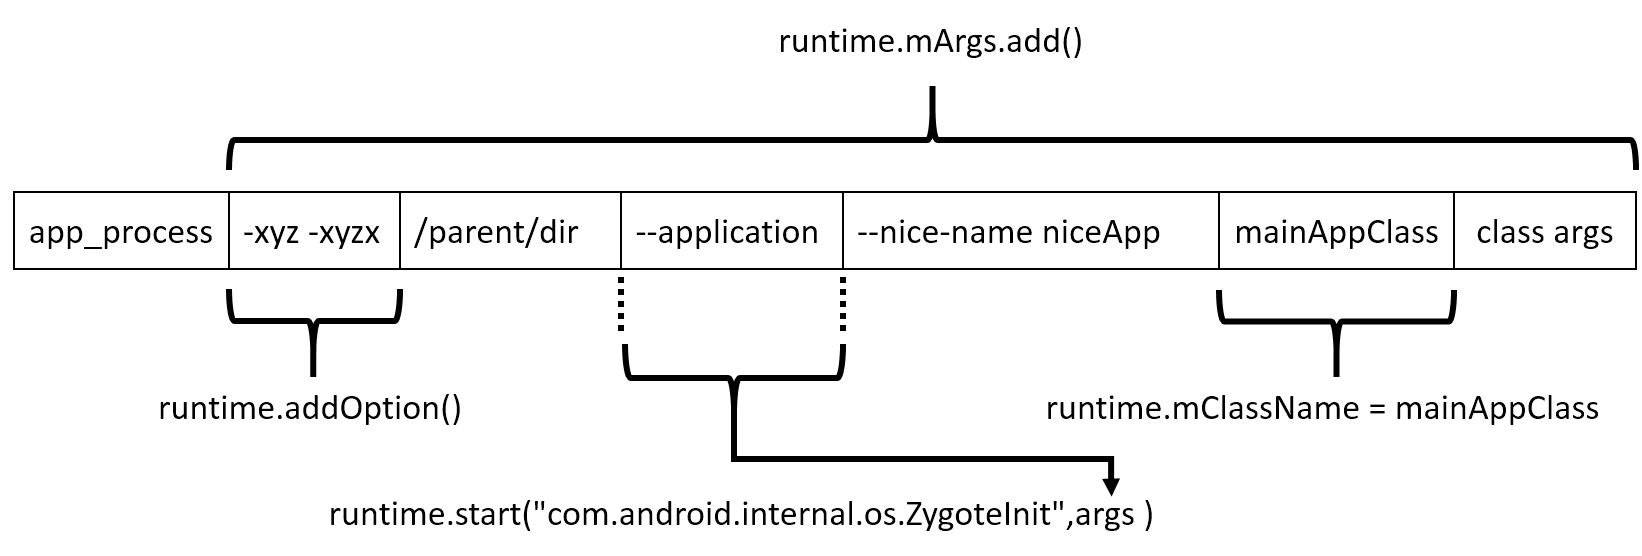
\includegraphics[width=\textwidth]{figures/app_process}
  \caption[App Process Argument Parsing]{App Process Argument Parsing}
  \label{fig:app_process}
\end{figure}


\section{Functionality of ``\code{AndroidRuntime.cpp}''}
The source file can be found at the path ``\code{/frameworks/base/core/jni/AndroidRuntime.cpp}''. As described in \autoref{section:app_main}, first the runtime constructor gets called followed by setting a few options as well as
the class name and all arguments and finally a call of the ``\code{start()}''
method. So a good start should be the constructor. It is quite short and
does reserve some space for options and is initializing a pointer to the object
itself.
The ``\code{start()}'' method does expect a class name (``.../ZygoteInit'') and a vector or args which is only one in this case. It follow
special log events in case of a system server start and a check if the root
dir ``\code{/system}'' does exist in the environment of linux.


